% !TEX root = ../thesis.tex
\makeatletter
\def\input@path{{../}}
\makeatother
\documentclass[../thesis.tex]{subfiles}
\begin{document}

\selectlanguage{english}
Pada bab ini akan dijabarkan hasil penelitian yang meliputi hasil pelatihan ulang model YOLOV3 baik secara statistik maupun secara visual, hasil perhitungan jumlah kendaraan tiap 5 menit oleh sistem dengan sampel durasi 1 jam, serta hasil pelatihan dan pengujian model LSTM untuk masing-masing variasi jumlah runtun data input dan output, jumlah lapisan LSTM, dan jumlah neuron tiap lapisan. Data hasil pengamatan akan dianalisa lebih lanjut.

Semua proses pengambilan data hasil penelitian dijalankan pada komputer Laboratorium Honeywell DTETI UGM dengan spesifikasi prosesor Intel Xeon E3-1225 v5 3.30 GHz.
RAM 8 GB, GPU NVIDIA GeForce GTX 1060 6GB dan sistem operasi Ubuntu 16.04 LTS.

\section{Objek Detektor}
\subsection{Deteksi Objek}
Untuk memberikan hasil deteksi objek yang bagus maka dilakukan pembuatan dataset sendiri sesuai dengan kondisi di lapangan. 
Jumlah total dataset adalah 1856 gambar dengan pembagian data pelatihan sebanyak 1688 gambar dan data uji sebanyak 168 gambar.
Pada proses pembuatan dataset ini dilakukan teknik augmentasi variasi tingkat saturasi dan kecerahan gambar. Teknik augmentasi seperti rotasi dan \textit{flip} tidak digunakan karena kondisi lalu lintas indonesia yang sangat padat sehingga 
terdapat banyak kendaraan yang memiliki daerah tumpang tindih.

Dataset akan dilatih menggunakan arsitektur YOLOV3 pada \textit{framework} darknet[link darknet]. Seperti yang telah dijelaskan, YOLOV3 membutuhkan 
9 buah anchor box. Anchor box dataset COCO tidak dapat digunakan dikarenakan dataset yang telah dibuat pada penelitian ini memiliki karakteristik yang jauh berbeda dengan COCO.
\textit{Framework} Darknet menyediakan fasilitas untuk membuat anchor box menggunakan algoritma K-NN. 9 Anchor box dari dataset pada penelitian ini adalah \\
\centerline{$[10x16, 12x27,  19x26,  16x42,  27x37,  24x58,  41x51, 47x76, 75x97]$}\

\begin{figure}[htp]
	\centering
	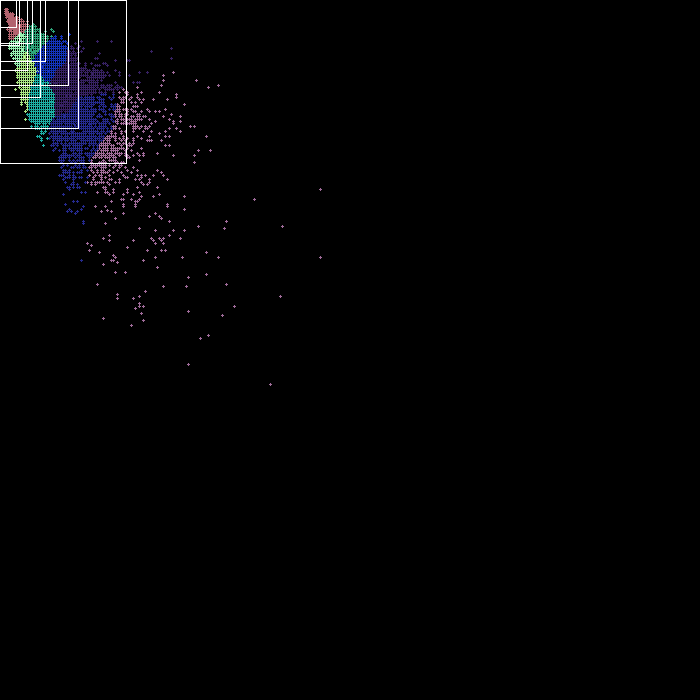
\includegraphics[scale=0.3]{anchor_new_full_dataset}
	\caption{Pembagian kluster pada anchor box}
	\label{anchor_dataset}
\end{figure}
dengan pembagian kluster seperti pada gambar \ref{anchor_dataset}. 9 anchor ini akan digunakan pada tiga lapisan YOLO terakhir.

Setelah anchor box berhasil dibuat, selanjutnya masuk tahap pelatihan dataset. Setting untuk proses pelatihan dilakukan pada file \textit{configuration} dimana Darknet akan membaca file ini. Untuk pelatihan pada penelitian ini menggunakan jumlah perulangan 12000 dengan 6 kelas sehingga setiap kelas akan dilatih sebanyak 2000 perulangan. 
\textit{Adaptive learning rate} juga diterapkan ketika perulangan telah mencapai 70\% dan 90\% dari total perulangan. Hal ini dilakukan agar informasi yang dilatih oleh jaringan semakin detail. Grafik pelatihan ditunjukan oleh gambar \ref{train_darknet}. Berdasarkan gambar tersebut, metric yang diamati selama pelatihan adalah mAP (\textit{mean average precision}) dan loss pelatihan.
\begin{figure}[htp]
	\centering
	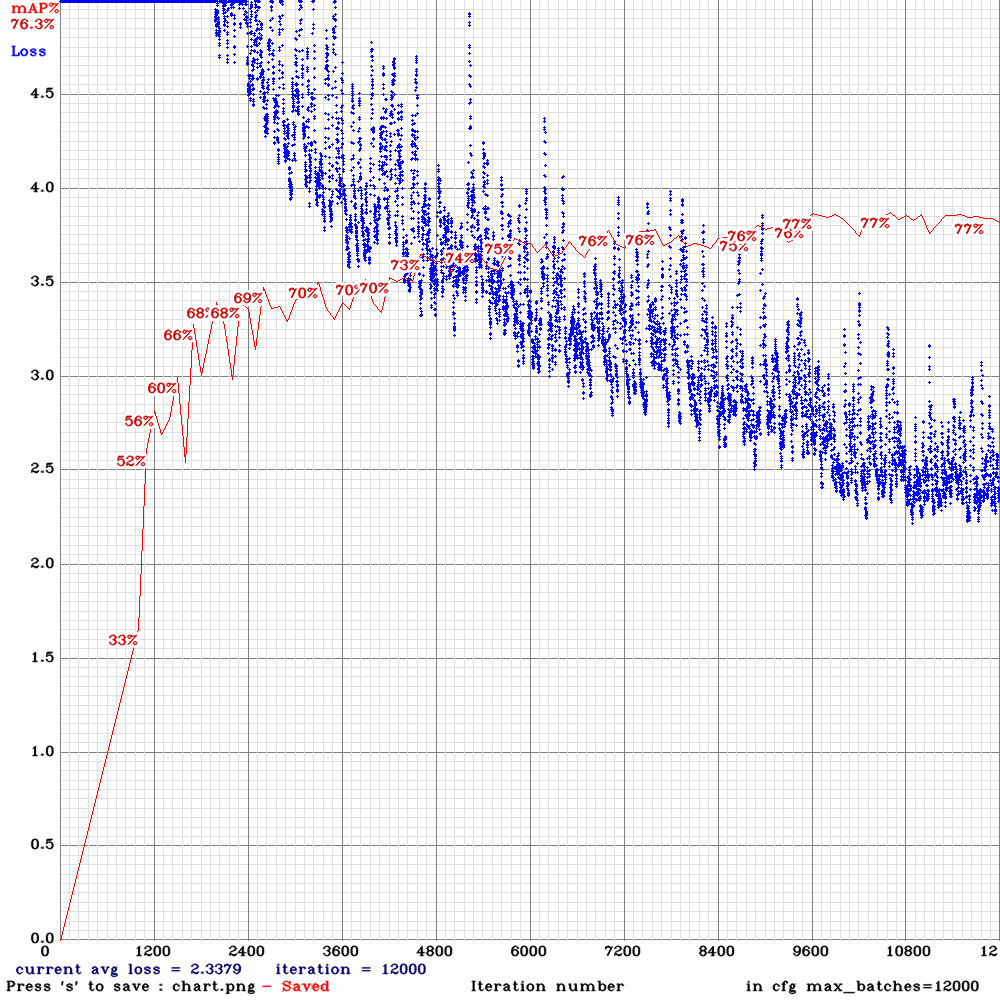
\includegraphics[scale=0.25]{new_full_dataset}
	\caption{Grafik proses pelatihan}
	\label{train_darknet}
\end{figure}
Dari gambar juga dapat diketahui bahwa model yang telah dilatih tidak mengalami \textit{overfitting}. Hal ini dapat dilihat dari grafik mAP (merah) yang terus mengalami kenaikan sedangkan grafik loss pelatihan (biru) mengalami penurunan.
Hasil pelatihan model pada masing-masing kelas dapat dilihat pada tabel \ref{Tabel_training}.
\begin{table}[htp]
\centering
\begin{tabular}{ cccccc }
	\hline 
	Kelas Id & Nama Kelas & AP & TP & FP\\
	\hline
	0& Person & 89.3\% & 10 & 2\\
	1 & Car & 94.93\% & 1624 & 171\\
	2 & Motorbike& 89.93\% &1092& 212 \\
	3 & Bus & 84.73\% & 27& 5 \\
	4 & Truck & 94.60\% & 191 & 27\\
	5 & Bicycle & 0.00\% &0 & 0 \\
\end{tabular}
\caption{Hasil pelatihan untuk tiap kelas}
\label{Tabel_training}
\end{table} 
Berdasarkan tabel tersebut dapat dilihat bahwa kelas yang memiliki \textit{average precision} terbesar adalah mobil, truck dan sepeda motor. Hal ini dikarenakan data latih atau kondisi lalu lintas Indonesia didominasi oleh tiga kelas tersebut, terutama mobil dan motor. 
Dari tabel \ref{Tabel_training} juga diketahui bahwa Total TP = 2944, Total FP = 417, dengan IoU = 68.22\% memberikan Total FN = 401. Maka dapat dicari nilai precision, recall dan F1-score nya berdasarkan persamaan \ref{Recall}, \ref{Precision}, \ref{F1_score}.
\begin{equation} \label{Precision}
	Precision = \frac{TP}{TP+FP} = \frac{2944}{2944+417} = 0.8759
\end{equation}

\begin{equation} \label{Recall}
	Recall = \frac{TP}{TP+FN} = \frac{2944}{2944+401} = 0.88
\end{equation}

\begin{equation} \label{F1_score}
	F1-score = 2*\frac{Precision * Recall}{Precision + Recall} = 2*\frac{0.88 * 0.8759}{0.88 + 0.8759} = 0.8779
\end{equation}

Perbandingan hasil antara model YOLOV3 yang telah dilatih menggunakan dataset sendiri dengan YOLOV3 asli secara visual seperti pada gambar \ref{compare_result}
\begin{figure}[htp]
	\centering
	\begin{subfigure}{0.35\textwidth}
	  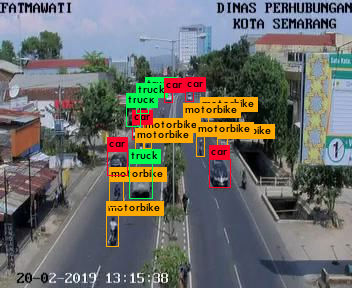
\includegraphics[width=\textwidth]{343_new}
	  \caption{model baru}
	  \label{new_model_result}
	\end{subfigure}
	\begin{subfigure}{0.35\textwidth}
	  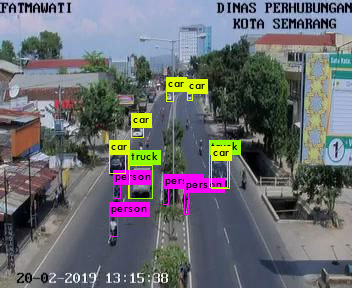
\includegraphics[width=\textwidth]{343_v3}
	  \caption{YOLOV3 asli}
	  \label{V3_result}
	\end{subfigure}
	\caption{Perbandingan hasil deteksi antara model baru dengan YOLOV3 asli}
	\label{compare_result}
  \end{figure}
Berdasarkan gambar tersebut dapat dilihat bahwa model yang baru memberikan hasil deteksi yang lebih bagus, terutama untuk kelas sepeda motor dimana YOLOV3 mengalami kesulitan untuk mendeteksi kelas ini secara baik.
Hasil deteksi dari model baru ini akan digunakan untuk melakukan \textit{tracking} dan perhitungan jumlah kendaraan.

\subsection{Perhitungan jumlah kendaraan}

Hasil perhitungan jumlah kendaraan oleh model yang telah dilatih kemudian dibandingkan dengan data acuan untuk mengetahui besaran error yang diberikan. Dalam penelitian ini, data acuan merupakan data hasil pengamatan secara langsung oleh pengamat yang diambil dari sampel 15 menit.
Metode mendapatkan data acuan ini dilakukan karena ATCS kota Semarang belum memiliki database yang berisi jumlah kendaraan tiap 5 menit. Untuk memberikan informasi yang lebih valid, pembuatan data acuan dilakukan oleh dua pengamat.
Hasil perbandingan antara perhitungan sistem dengan pengamat dapat dilihat pada tabel \ref{Count_result}. 
\begin{table}[htp]
\centering
\begin{tabular}{|c|c|c|c|}
	\hline 
	\multirow{2}{*}{\textbf{5 menit ke-}} & \multicolumn{2}{c|}{\textbf{Grountruth}} &  \multirow{2}{*}{\textbf{Hasil perhitungan sistem}}\\ \cline{2-3}
	& Orang 1& Orang 2 &\\
	\hline
	1& 212 & 206 & 184\\
	2 & 270 & 278 & 254\\
	3 & 200 & 192 & 177\\
	4 & 227 & 235 & 204 \\
	5 & 223 & 232 & 202 \\
	6 & 248 & 241 & 235 \\
	7 & 232 & 208 & 217 \\
	8 & 235 & 241 & 213 \\
	9 & 269 & 273 & 248 \\
	10 & 265 & 271 & 243 \\
	11 & 229 & 235 & 206 \\
	\hline
\end{tabular}
\caption{Perbandingan hasil perhitungan sistem dengan \textit{groundtruth}}
\label{Count_result}
\end{table} 
Berdasarkan tabel \ref{Count_result} diketahui bahwa rata-rata error perhitungan oleh sistem tiap 5 menit sebesar 20 kendaraan.

\section{Prediksi arus lalu lintas menggunakan LSTM}
Model yang telah dilatih digunakan untuk membuat dataset untuk jaringan LSTM.
Perhitungan jumlah kendaraan menggunakan model yang telah ada dilakukan secara \textit{live streaming} dengan memanfaatkan layanan ATCS dishub kota Semarang. Lokasi yang dipilih adalah jalan Fatmawati. Perhitungan dilakukan setiap 5 menit mulai dari pukul 07.00 sampai dengan 17.45 selama 2 minggu . 
Data hasil perhitungan ini disimpan dalam file .csv dan akan digunakan baik untuk proses pelatihan maupun proses pengujian LSTM.

Berdasarkan skema pengambilan data jumlah kendaraan diatas, diperoleh data dengan jumlah 1430 data untuk 11 hari sehingga per hari terdapat 130 data.
Proses pengolahan data yang dilakukan yaitu membagi data menjadi data latih dan data uji. Pada penelitian ini data latih sebanyak 1170 data (9 hari) dan data uji sebanyak 260 data (2 hari)
Untuk proses pelatihan sendiri akan memvariasikan beberapa parameter yaitu jumlah lapisan LSTM, jumlah neuron tiap lapisan, jumlah data input, serta jumlah data output LSTM. 
Jumlah lapisan yang akan digunakan yaitu 1,2,3, dan 4 LSTM, jumlah neuron yang digunakan 50 dan 100, jumlah data input yang digunakan adalah 130, 260 dan 390, sedangkan jumlah output yang digunakan adalah 130, 65, dan 1. Masing-masing 
variasi akan diamati nilai RMSE, dan MAPE nya. Variasi yang memberikan nilai RMSE dan MAPE terendah akan dipakai untuk implementasi di dashboard.

Setelah melakukan proses pelatihan diperoleh model sebanyak variasi. Nilai RMSE dan MAPE masing-masing model dapat dilihat pada tabel \ref{1LSTM_result}, \ref{2LSTM_result}, dan \ref{3LSTM_result}.
\begin{table}[htp]
\centering
\begin{tabular}{|c|c|c|c|c|c|}
	\hline 
	\multirow{3}{*}{\textbf{Input LSTM}} & \multirow{3}{*}{\textbf{Output LSTM}} & \multicolumn{4}{c|}{\textbf{1 LSTM}} \\ \cline{3-6}
	&  & \multicolumn{2}{c|}{50}& \multicolumn{2}{c|}{100} \\ \cline{3-6}
	& & RMSE & MAPE& RMSE & MAPE\\
	\hline
	\multirow{3}{*}{130} & 130 & 30.34& 11.316\%& 28.153 & 10.878\%\\
	& 65 & 31.782 & 11.628\% & 26.919 & 11.353\% \\
	& 1 & 28.468 & 11.491\% & 27.669 & 11.614\% \\
	\hline
	\multirow{3}{*}{260} & 130 & 29.142 & 11.67\%  & 27.716 & 10.864\%\\
	& 65 & 29.784 & 11.458\% & 29.830 & 12.022\%\\
	& 1 & 28.267 & 11.389\% & 27.883 & 11.440\% \\
	\hline
	\multirow{3}{*}{390} & 130 & 32.301 & 12.446\% & 30.567 & 11.416\% \\
	& 65 & 32.015 & 12.541\% & 30.664 & 12.220\% \\
	& 1 & 28.332 & 11.417\% & 27.65 & 11.542\% \\
	\hline
\end{tabular}
\caption{Nilai RMSE dan MAPE menggunakan 1 LSTM}
\label{1LSTM_result}
\end{table} 

\begin{table}[htp]
	\centering
	\begin{tabular}{|c|c|c|c|c|c|}
		\hline 
		\multirow{3}{*}{\textbf{Input LSTM}} & \multirow{3}{*}{\textbf{Output LSTM}} & \multicolumn{4}{c|}{\textbf{2 LSTM}} \\ \cline{3-6}
		&  & \multicolumn{2}{c|}{50;50}& \multicolumn{2}{c|}{100;100} \\ \cline{3-6}
		& & RMSE & MAPE& RMSE & MAPE\\
		\hline
		\multirow{3}{*}{130} & 130 & 32.022 & 12.920\% & 29.610 & 10.964 \%\\
		& 65 & 29.484 & 12.051\%& 39.009\% & 15.242\% \\
		& 1 & 27.571 & 12.062\% & 27.787 & 12.180\% \\
		\hline
		\multirow{3}{*}{260} & 130 & 30.109 & 11.572\% & 28.770\% & 11.107\% \\
		& 65 & 28.983 & 11.204\% & 28.443 & 11.898\% \\
		& 1 & 27.165 & 11.66\% & 27.565 & 12.145\% \\
		\hline
		\multirow{3}{*}{390} & 130 & 27.68 & 11.03\% & 28.625 & 11.958\% \\
		& 65 & 31.245 & 11.610\% & 31.512 & 12.579\% \\
		& 1 & 27.377 & 11.55\% & 27.833 & 11.658\% \\
		\hline
	\end{tabular}
	\caption{Nilai RMSE dan MAPE menggunakan 2 LSTM}
	\label{2LSTM_result}
	\end{table} 

\begin{table}[htp]
	\centering
	\begin{tabular}{|c|c|c|c|c|c|}
		\hline 
		\multirow{3}{*}{\textbf{Input LSTM}} & \multirow{3}{*}{\textbf{Output LSTM}} & \multicolumn{4}{c|}{\textbf{3 LSTM}} \\ \cline{3-6}
		&  & \multicolumn{2}{c|}{50;50;50}& \multicolumn{2}{c|}{100;100;100} \\ \cline{3-6}
		& & RMSE & MAPE& RMSE & MAPE\\
		\hline
		\multirow{3}{*}{130} & 130 & 34.268 & 12.801\% & 36.555 & 14.052\% \\
		& 65 & 29.479 & 11.915\% & 33.423 & 14.439\% \\
		& 1 & 27.390 & 12.116\% & 27.346 & 12.008\% \\
		\hline
		\multirow{3}{*}{260} & 130 & 26.059 & 11.075\% & 25.933 & 10.362\% \\
		& 65 & 26.428 & 10.729\% & 37.004 & 14.642\% \\
		& 1 & 26.583 & 11.144\% &  27.557 & 11.268\% \\
		\hline
		\multirow{3}{*}{390} & 130 & 29.889 & 11.668\% & 35.517 & 13.226\% \\
		& 65 & 38.861 & 16.415\% & 38.512 & 14.477\% \\
		& 1 & 27.972 & 11.150\% & 27.392 & 11.752\% \\
		\hline
	\end{tabular}
	\caption{Nilai RMSE dan MAPE menggunakan 3 LSTM}
	\label{3LSTM_result}
	\end{table} 

% \begin{table}[htp]
% 	\centering
% 	\begin{tabular}{|c|c|c|c|c|c|}
% 		\hline 
% 		\multirow{3}{*}{\textbf{Input LSTM}} & \multirow{3}{*}{\textbf{Output LSTM}} & \multicolumn{4}{c|}{\textbf{4 LSTM}} \\ \cline{3-6}
% 		&  & \multicolumn{2}{c|}{50;50;50;50}& \multicolumn{2}{c|}{100;100;100;100} \\ \cline{3-6}
% 		& & RMSE & MAPE& RMSE & MAPE\\
% 		\hline
% 		\multirow{3}{*}{130} & 130 & & & & \\
% 		& 65 & & & & \\
% 		& 2 & & & & \\
% 		\hline
% 		\multirow{3}{*}{260} & 130 & & & & \\
% 		& 65 & & & & \\
% 		& 2 & & & & \\
% 		\hline
% 		\multirow{3}{*}{390} & 130 & & & & \\
% 		& 65 & & & & \\
% 		& 2 & & & & \\
% 		\hline
% 	\end{tabular}
% 	\caption{Nilai RMSE dan MAPE menggunakan 4 LSTM}
% 	\label{4LSTM_result}
% 	\end{table} 

Berdasarkan tabel \ref{1LSTM_result}, \ref{2LSTM_result}, dan \ref{3LSTM_result}, dapat diketahui karakteristik jaringan LSTM sebagai berikut:
\begin{enumerate}
	\item Dengan ukuran input yang sama, semakin kecil ukuran output maka semakin kecil pula RMSE dan MAPE yang diberikan. 
	\item Dengan ukuran output yang sama penambahan jumlah input membuat RMSE dan MAPE semakin berkurang. Namun dengan ukuran input 390, RMSE dan MAPE justru lebih besar dibandingkan input 260. Hal ini dikarenakan kurangnya data latih untuk input 390 sehingga LSTM tidak dapat mempelajari secara maksimal karakteristik data. Dengan data input sebesar 390  dan misalkan jumlah output 1, berarti hanya terdapat 3 runtun data latih dengan bentuk (3, 390, 1). Apabila data latih ini digunakan untuk membuat data $train\_x$ dengan sistem \textit{sliding window} maka hanya didapatkan data $train\_x$ sebanyak (780,390,1). Jumlah runtun data ini lebih sedikit dibandingkan dengan ukuran input 260 dan 130 untuk jumlah output yang sama. Dengan jumlah output yang sama yaitu 1, input 260 memberikan jumlah data $train\_x$ sebanyak (1040, 260, 1) sedangkan dengan input 130 memberikan data $train\_x$ sebanyak (1040,130,1).
	\item Dengan mengkombinasikan antara jumlah output, jumlah input, jumlah lapisan LSTM dan jumlah neuron tiap lapisan secara proporsional dapat dibuat sebuah model yang optimal  
\end{enumerate}

Berdasarkan tabel, diketahui bahwa untuk output 130 model terbaik ditemukan pada kombinasi jumlah input = 260, jumlah lapisan LSTM = 3, dan jumlah neuron tiap lapisan = 100 dengan RMSE sebesar 25.933 dan MAPE 10.362\%. Untuk output 65 model terbaik ditemukan pada kombinasi jumlah input = 260, jumlah lapisan LSTM = 3, dan jumlah neuron tiap lapisan = 50 dengan RMSE sebesar 26.428 dan MAPE 10.729\%.
Sedangkan untuk output 130 model terbaik ditemukan pada kombinasi jumlah input = 260, jumlah lapisan LSTM = 3, dan jumlah neuron tiap lapisan = 50 dengan RMSE sebesar 26.583 dan MAPE 11.144\%.

Hasil perbandingan antara output model dengan data uji ditunjukkan oleh gambar \ref{out_130}, \ref{out_65}, \ref{out_1}.
\begin{figure}[htp]
	\centering
	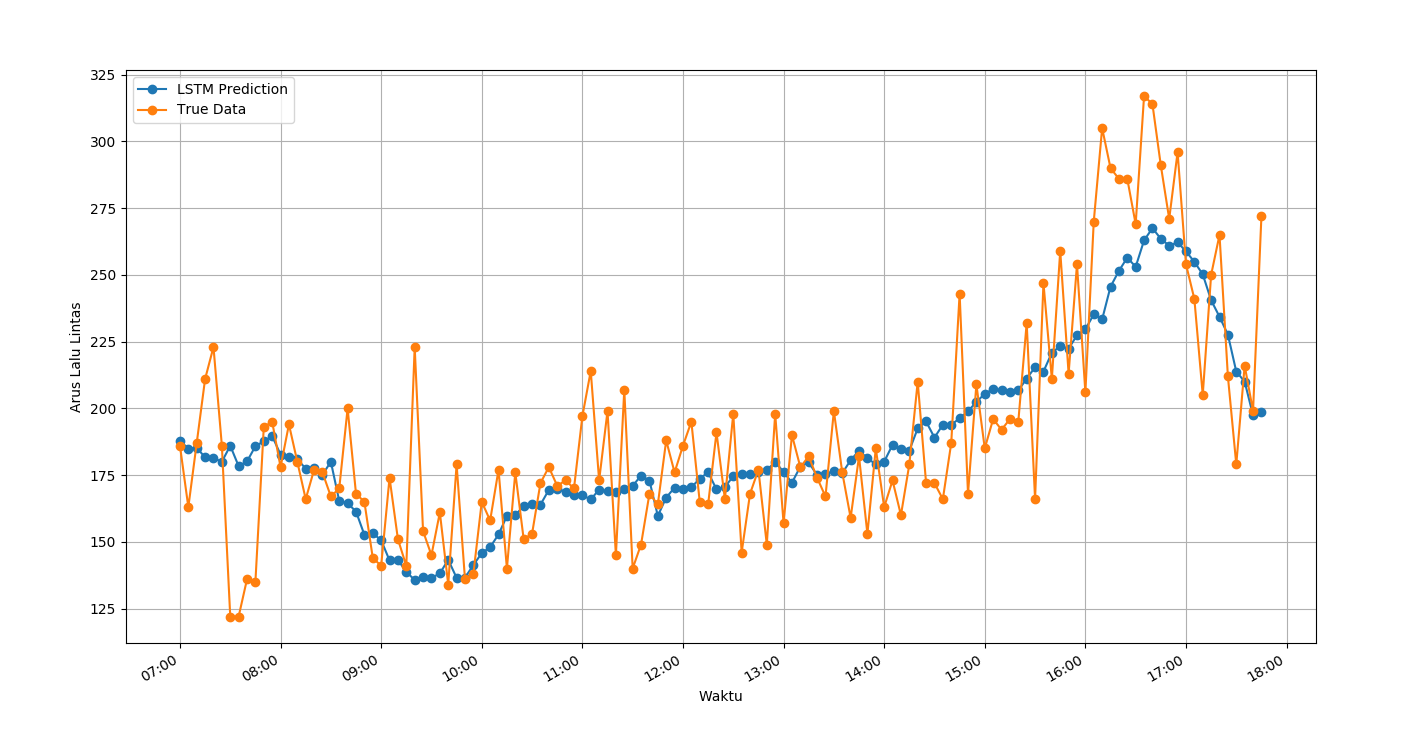
\includegraphics[scale=0.3]{out_130}
	\caption{Hasil prediksi model dengan output 130}
	\label{out_130}
\end{figure}

\begin{figure}[htp]
	\centering
	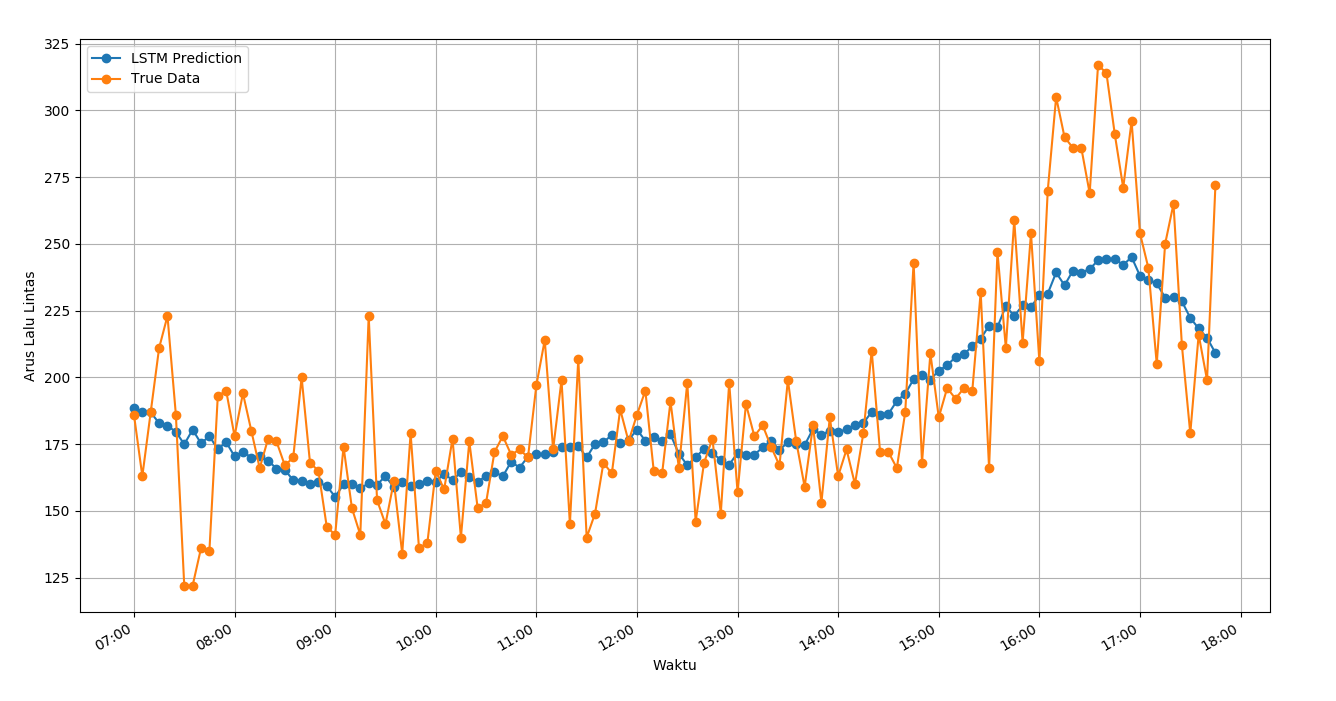
\includegraphics[scale=0.3]{out_65}
	\caption{Hasil prediksi model dengan output 65}
	\label{out_65}
\end{figure}

\begin{figure}[htp]
	\centering
	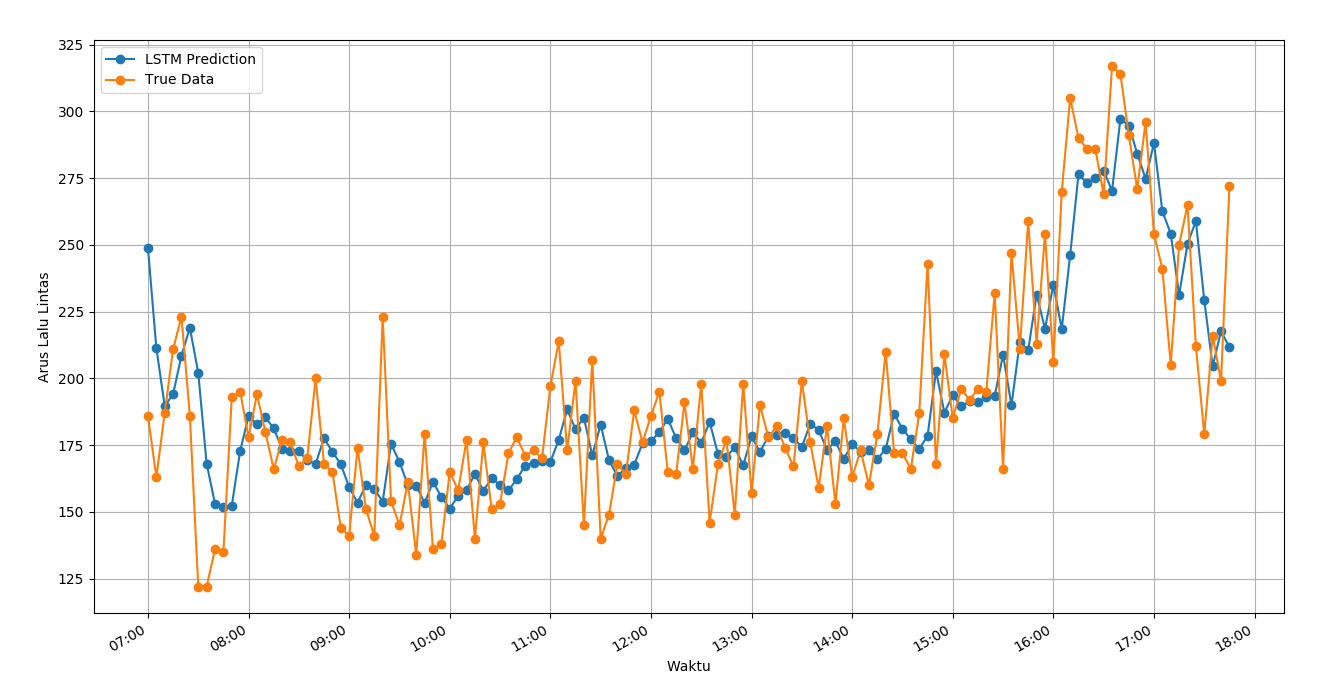
\includegraphics[scale=0.3]{out_1}
	\caption{Hasil prediksi model dengan output 1}
	\label{out_1}
\end{figure}
Berdasarkan gambar tersebut dapat diketahui bahwa meskipun nilai RMSE dan MAPE yang dimiliki oleh model dengan output 1 secara statistika lebih buruk daripada model dengan output 130 dan 65, namun secara visual model dengan output 1 mampu mengikuti tren dari data uji lebih baik. Hal ini dikarenakan dengan jumlah output yang semakin sedikit, maka model akan semakin presisi untuk mempelajari karakteristik data namun
akan membuuhkan waktu lama untuk melakukan prediksi. 

\section{Perancangan dashboard}
Pada perancangan ini akan dibuat 2 buah dashboard yaitu dashboard utama dan dashboard kedua. Skema perancangan dashboard secara keseluruhan seperti pada gambar \ref{all_system}.
% \begin{figure}[htp]
% 	\centering
% 	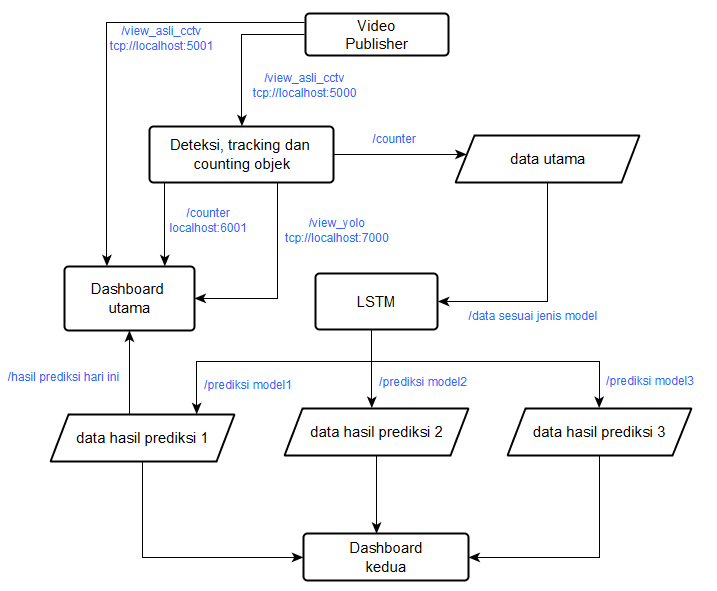
\includegraphics[scale=0.6]{all_system}
% 	\caption{Skema perancangan dashboard yang dilakukan}
% 	\label{all_system}
% \end{figure}

Dari gambar \ref{all_system}, tampak bahwa dashboard utama akan menampilkan data berupa view asli dari CCTV, view CCTV setelah dikenai objek detektor, grafik perhitungan jumlah kendaraan, dan hasil prediksi untuk hari yang bersangkutan.
Sedangkan dashboard kedua akan mengakses data hasil prediksi 1, data hasil prediksi 2 dan data hasil prediksi 3. Data-data ini berada pada file csv terpisah dan mengandung data prediksi hingga 6 hari kedepan. Dengan kata lain dashboard kedua digunakan
apabila seseorang ingin melihat prediksi arus lalu lintas untuk 2 hari bahkan 6 hari kedepan.

\end{document}